\documentclass[11pt,a4paper]{article}
\usepackage[T5,T1]{fontenc}
\usepackage[utf8]{inputenc}
\usepackage{vntex}
\usepackage[english]{babel}
\usepackage[a4paper,margin=2.25cm,headheight=40pt,footskip=28pt]{geometry}
\usepackage{lmodern}
\usepackage{graphicx,xcolor}
\usepackage{booktabs,tabularx,longtable,array,multirow}
\usepackage{amsmath,amssymb}
\usepackage{enumitem}
\usepackage{fancyhdr,lastpage}
\usepackage{float}
\usepackage{caption}
\usepackage{comment}
\usepackage{hyperref}
\usepackage{listings}
\usepackage{microtype}
\usepackage{titlesec}

\hypersetup{colorlinks=true,linkcolor=black,urlcolor=black,citecolor=black,pdftitle={Resume Analyzer},pdfauthor={NLP Course Project Group}}
\definecolor{ink}{HTML}{000000}
\definecolor{accent}{HTML}{000000}
\definecolor{pale}{HTML}{FFFFFF}
\definecolor{muted}{HTML}{000000}
\definecolor{placeholderblue}{HTML}{005B9D}
\setlength{\parindent}{1.1em}
\setlength{\parskip}{0.24em}
\setcounter{tocdepth}{2}
\setlist[itemize]{leftmargin=1.5em,itemsep=0.13em,topsep=0.3em}
\setlist[enumerate]{leftmargin=1.7em,itemsep=0.12em,topsep=0.3em}
\renewcommand{\arraystretch}{1.15}
\titleformat{\section}{\Large\bfseries\color{ink}}{\thesection.}{0.65em}{}
\titleformat{\subsection}{\large\bfseries\color{accent}}{\thesubsection}{0.65em}{}
\captionsetup{font=small,labelfont=bf}

\pagestyle{fancy}
\fancyhf{}
\fancyhead[L]{
\includegraphics[height=0.43cm]{hcmut.png}\hspace{0.2cm}\footnotesize\textbf{HCMUT -- Faculty of Computer Science and Engineering}}
\fancyfoot[L]{\footnotesize Natural Language Processing | Course Project: Resume Analyzer}
\fancyfoot[R]{\footnotesize Page \thepage}
\renewcommand{\headrulewidth}{0.3pt}

\lstdefinestyle{command}{basicstyle=\ttfamily\footnotesize,frame=single,backgroundcolor=\color{white},breaklines=true,columns=fullflexible,keepspaces=true,showstringspaces=false}
\lstset{style=command}
\newcommand{\code}[1]{{\ttfamily\detokenize{#1}}}
\newcommand{\statusnote}[1]{\par\noindent\begingroup\setlength{\fboxsep}{8pt}\colorbox{pale}{\parbox{\dimexpr\linewidth-2\fboxsep\relax}{\small #1}}\endgroup\par}

\begin{document}

\hypersetup{pageanchor=false}
\begin{titlepage}
\centering
{\large VIETNAM NATIONAL UNIVERSITY -- HO CHI MINH CITY\par}
\vspace{0.25cm}
{\Large\bfseries HO CHI MINH CITY UNIVERSITY OF TECHNOLOGY\par}
{\large Faculty of Computer Science and Engineering\par}
\vspace{1.4cm}

\includegraphics[width=3.3cm]{hcmut.png}\par
\vspace{1.15cm}
{\Large\bfseries NATURAL LANGUAGE PROCESSING\par}
{\normalsize Semester I -- Academic Year 2026--2027\par}
\vspace{0.65cm}
\textcolor{accent}{\rule{0.9\linewidth}{1.2pt}}\par
\vspace{0.4cm}
{\Huge\bfseries\color{ink} Resume Analyzer\par}
\vspace{0.45cm}
{\Large Course Project Report\par}
\vspace{0.4cm}
\textcolor{accent}{\rule{0.9\linewidth}{1.2pt}}\par
\vspace{1.0cm}
\begin{tabular}{rl}
\textbf{Course:} & Natural Language Processing\\
\textbf{Project:} & Resume Analyzer\\
\textbf{Supervisor:} & TS. Trương Vĩnh Lân\\
\end{tabular}
\vspace{0.72cm}

{\large\bfseries Team Members\par}
\vspace{0.20cm}
{\small
\renewcommand{\arraystretch}{1.35}
\begin{tabular}{@{}c p{6.2cm} p{2.8cm} c@{}}
\toprule
\textbf{No.} & \textbf{Full Name} & \textbf{Student ID} & \textbf{Role}\\
\midrule
1 & Kriti Sharma & {[Student ID]} & {[Role]}\\
2 & Nguyễn Hà Bảo Phúc & {[Student ID]} & {[Role]}\\
3 & Phạm Trương Hoàng Long & 2452700 & {[Role]}\\
4 & Yuvaan Chottani & {[Student ID]} & {[Role]}\\
\bottomrule
\end{tabular}
}
\vfill
{Ho Chi Minh City, November 2026\par}
\end{titlepage}

\pagenumbering{roman}
\tableofcontents
\clearpage
\pagenumbering{arabic}
\hypersetup{pageanchor=true}

\section{Introduction}
\subsection{Problem Statement \& Motivation}
\par\noindent\textit{[TODO: Describe the real-world problem of automated resume classification and job matching, and the motivation for this project.]}

\subsection{Objectives \& Scope}
\par\noindent\textit{[TODO: Summarize the project objectives, 24-class classification formulation, and system scope.]}

\section{Related Work}
\subsection{Automated Resume Screening \& Text Classification}
\par\noindent\textit{[TODO: Briefly review prior work on resume classification and recruitment NLP systems.]}

\subsection{Text Representations \& Neural Architectures}
\par\noindent\textit{[TODO: Briefly review sparse representations (BoW, TF-IDF), static embeddings (GloVe), recurrent/convolutional models (BiLSTM, BiGRU, TextCNN), and pretrained Transformers (DistilBERT).]}

\section{Dataset Description}
\subsection{Data Source \& Collection}
The dataset used in this project is the public \textbf{Resume Dataset} from Kaggle (\texttt{snehaanbhawal/\allowbreak resume-dataset}), comprising \textbf{2,484} English curriculum vitae (CVs) categorized into \textbf{24} occupational classes. Each CV is labeled with a single job category (\code{Category}) representing the target domain of the entire document, while internal sections such as skills, work experience, and education appear within the unstructured resume body.

The raw source file (\code{raw/Resume.csv}) contains four columns: \code{ID}, \code{Resume_str}, \code{Resume_html}, and \code{Category}. During preprocessing, a \code{split} column is added to track partition membership (\code{train}, \code{val}, \code{test}, or \code{excluded}), and \code{text} holds the corresponding processed CV wording. Table~\ref{tab:dataset_schema} summarizes the field types, and Table~\ref{tab:file_schemas} details the exact column layout across all raw, processed, and split files.

\begin{table}[H]
\centering
\small
\renewcommand{\arraystretch}{1.25}
\begin{tabularx}{\linewidth}{@{}l l X@{}}
\toprule
\textbf{Type} & \textbf{Column} & \textbf{Meaning}\\
\midrule
String key & \code{ID} & Unique CV identifier shared across all raw, processed, and split tables.\\
Categorical & \code{Category} & Source job category label (24 classes, e.g., \code{ACCOUNTANT}).\\
Categorical & \code{split} & Partition assignment: \code{train}, \code{val}, \code{test}, or \code{excluded}.\\
Plain text & \code{Resume_str}, \code{text} & Original plain-text CV wording or its preprocessed text variant.\\
HTML text & \code{Resume_html} & Original HTML markup used to locate and align the opening header.\\
\bottomrule
\end{tabularx}
\caption{Dataset field types and column definitions.}
\label{tab:dataset_schema}
\end{table}

\begin{table}[H]
\centering
\small
\renewcommand{\arraystretch}{1.2}
\begin{tabularx}{\linewidth}{@{}l X c@{}}
\toprule
\textbf{File} & \textbf{Columns in order} & \textbf{Count}\\
\midrule
\code{raw/Resume.csv} & \code{ID}, \code{Resume_str}, \code{Resume_html}, \code{Category} & 4\\
\code{processed/raw_no_header.csv} & \code{ID}, \code{Category}, \code{split}, \code{text} & 4\\
\code{processed/light.csv} & \code{ID}, \code{Category}, \code{split}, \code{text} & 4\\
\code{processed/classical.csv} & \code{ID}, \code{Category}, \code{split}, \code{text} & 4\\
\code{processed/stemmed.csv} & \code{ID}, \code{Category}, \code{split}, \code{text} & 4\\
\code{processed/lemmatized.csv} & \code{ID}, \code{Category}, \code{split}, \code{text} & 4\\
\code{split/train.csv} & \code{ID}, \code{Category} & 2\\
\code{split/val.csv} & \code{ID}, \code{Category} & 2\\
\code{split/test.csv} & \code{ID}, \code{Category} & 2\\
\bottomrule
\end{tabularx}
\caption{Column schemas across raw, processed, and split CSV files (all processed files retain all 2,484 source IDs).}
\label{tab:file_schemas}
\end{table}

\subsection{Dataset Size, Cleaning \& Class Distribution}
Before model training, the 2,484 raw records undergo an integrity and duplicate audit (\code{src/prepare_data.py} and \texttt{src/long\_\-preprocessing/splits.py}) to prevent train--test leakage:
\begin{itemize}
    \item \textbf{Excluded records:} After NFKC Unicode normalization, case-folding, and whitespace folding, \textbf{1} blank CV and \textbf{2} exact-duplicate copies are excluded (\code{split = excluded} in the preprocessing outputs), leaving \textbf{2,481} unique valid resumes. Conflicting-label exact duplicates are also checked and quarantined. All 2,484 IDs are retained in the prepared CSVs for full auditability.
    \item \textbf{Frozen stratified split:} The 2,481 unique resumes are partitioned using a stratified 80\% / 10\% / 10\% split (\code{random_state = 42}), yielding \textbf{1,984} training, \textbf{248} validation, and \textbf{249} test samples. Freezing this exact \code{sample_id} membership across all classical, RNN/CNN, and Transformer models ensures fair, paired comparisons. In addition, \code{splits.py} audits near-duplicates using 5-word shingles (Jaccard threshold $\ge 0.85$, \code{MIN_SHINGLES = 25}) and verifies via \code{prepare_no_title.py} that the header-removed dataset preserves the exact same 1,984 / 248 / 249 sample IDs and labels.
\end{itemize}

As shown in Figure~\ref{fig:class_dist}, the dataset exhibits moderate class imbalance across its 24 categories. Most categories contain between 96 and 120 resumes, led by \code{INFORMATION-TECHNOLOGY} and \code{BUSINESS-DEVELOPMENT} with 120 resumes each, whereas minority categories such as \code{AGRICULTURE} (63), \code{AUTOMOBILE} (36), and \code{BPO} (22) have substantially fewer samples. Because standard Accuracy can be dominated by majority classes under this imbalance, \textbf{Macro-F1} is adopted as the primary evaluation metric (assigning equal weight to all 24 classes), and models use class weighting during training. Figure~\ref{fig:split_by_cat} confirms that the 80/10/10 split preserves class proportions consistently across all 24 categories.

\begin{figure}[H]
\centering
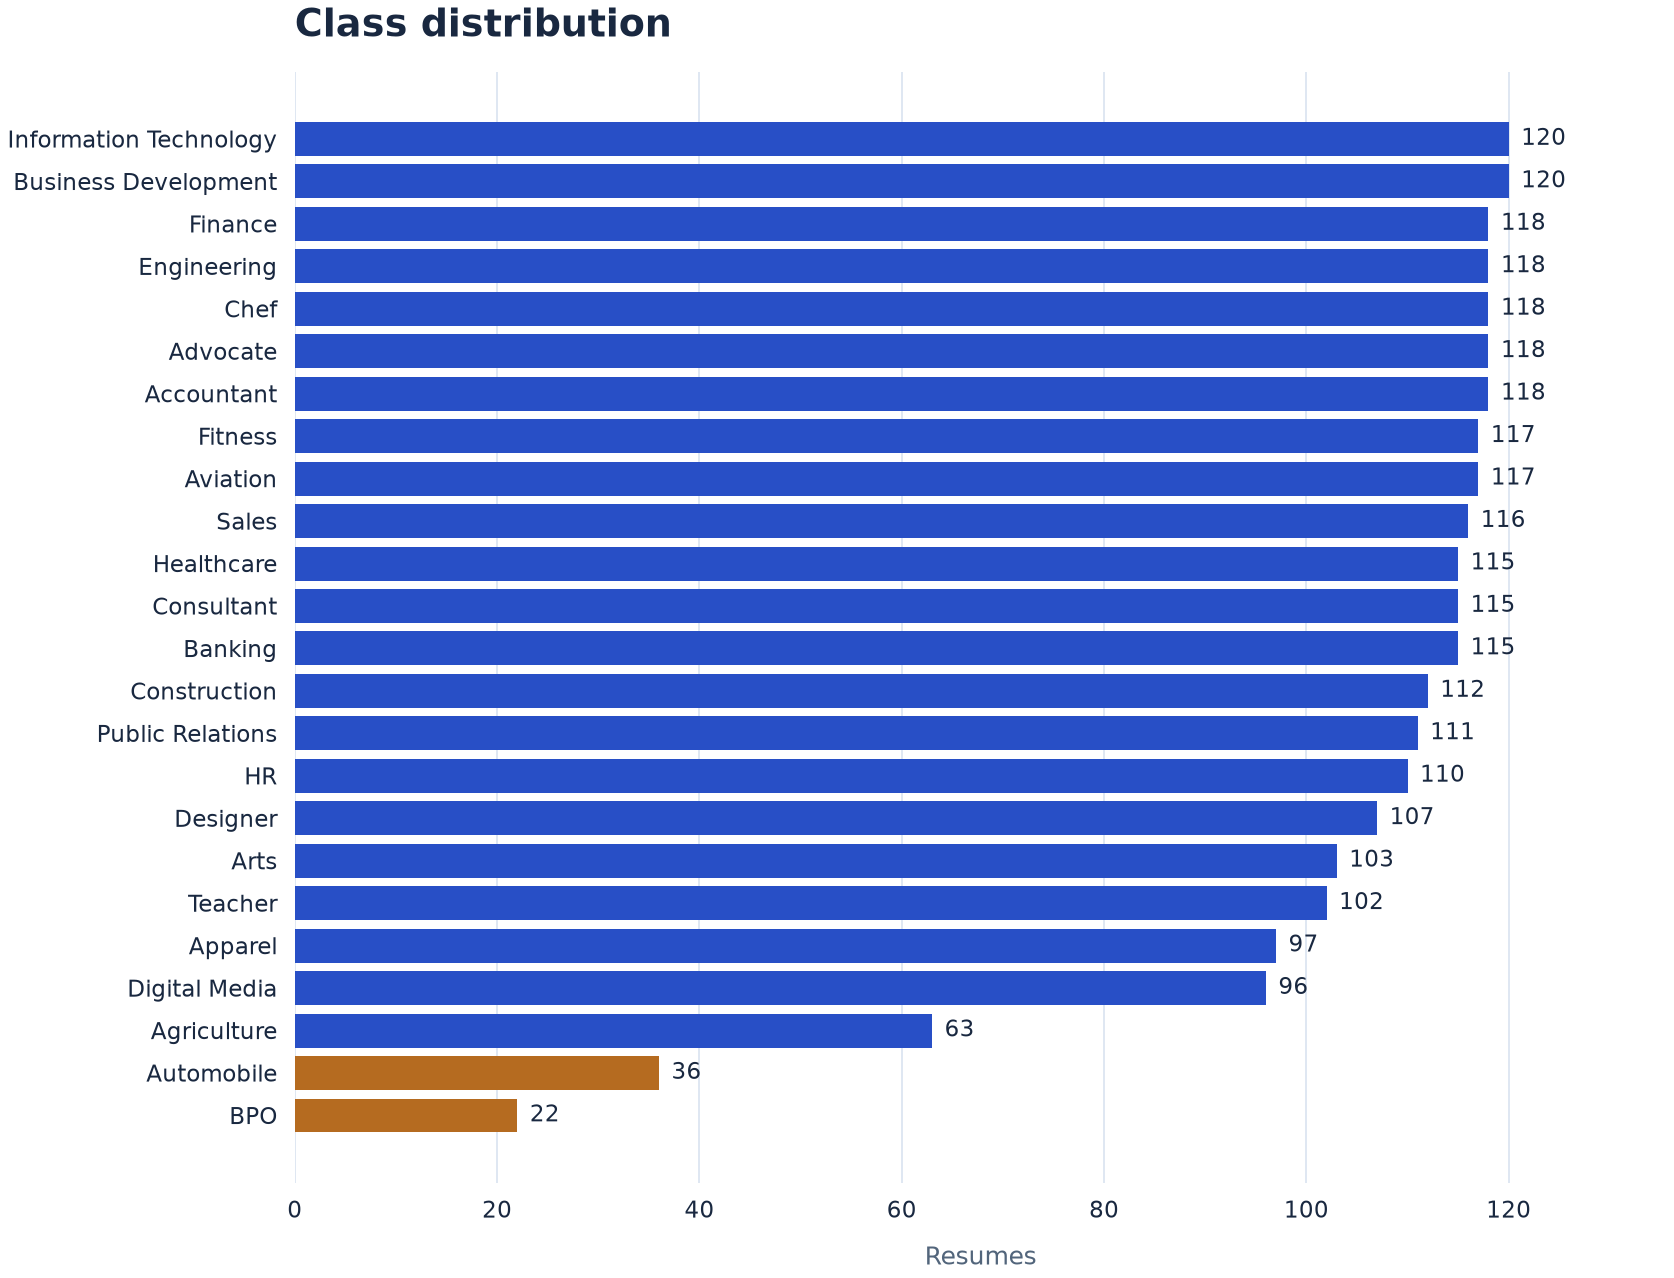
\includegraphics[width=0.92\linewidth]{charts/class_distribution.png}
\caption{Distribution of resumes across the 24 occupational categories (2,484 total records).}
\label{fig:class_dist}
\end{figure}

\begin{figure}[H]
\centering
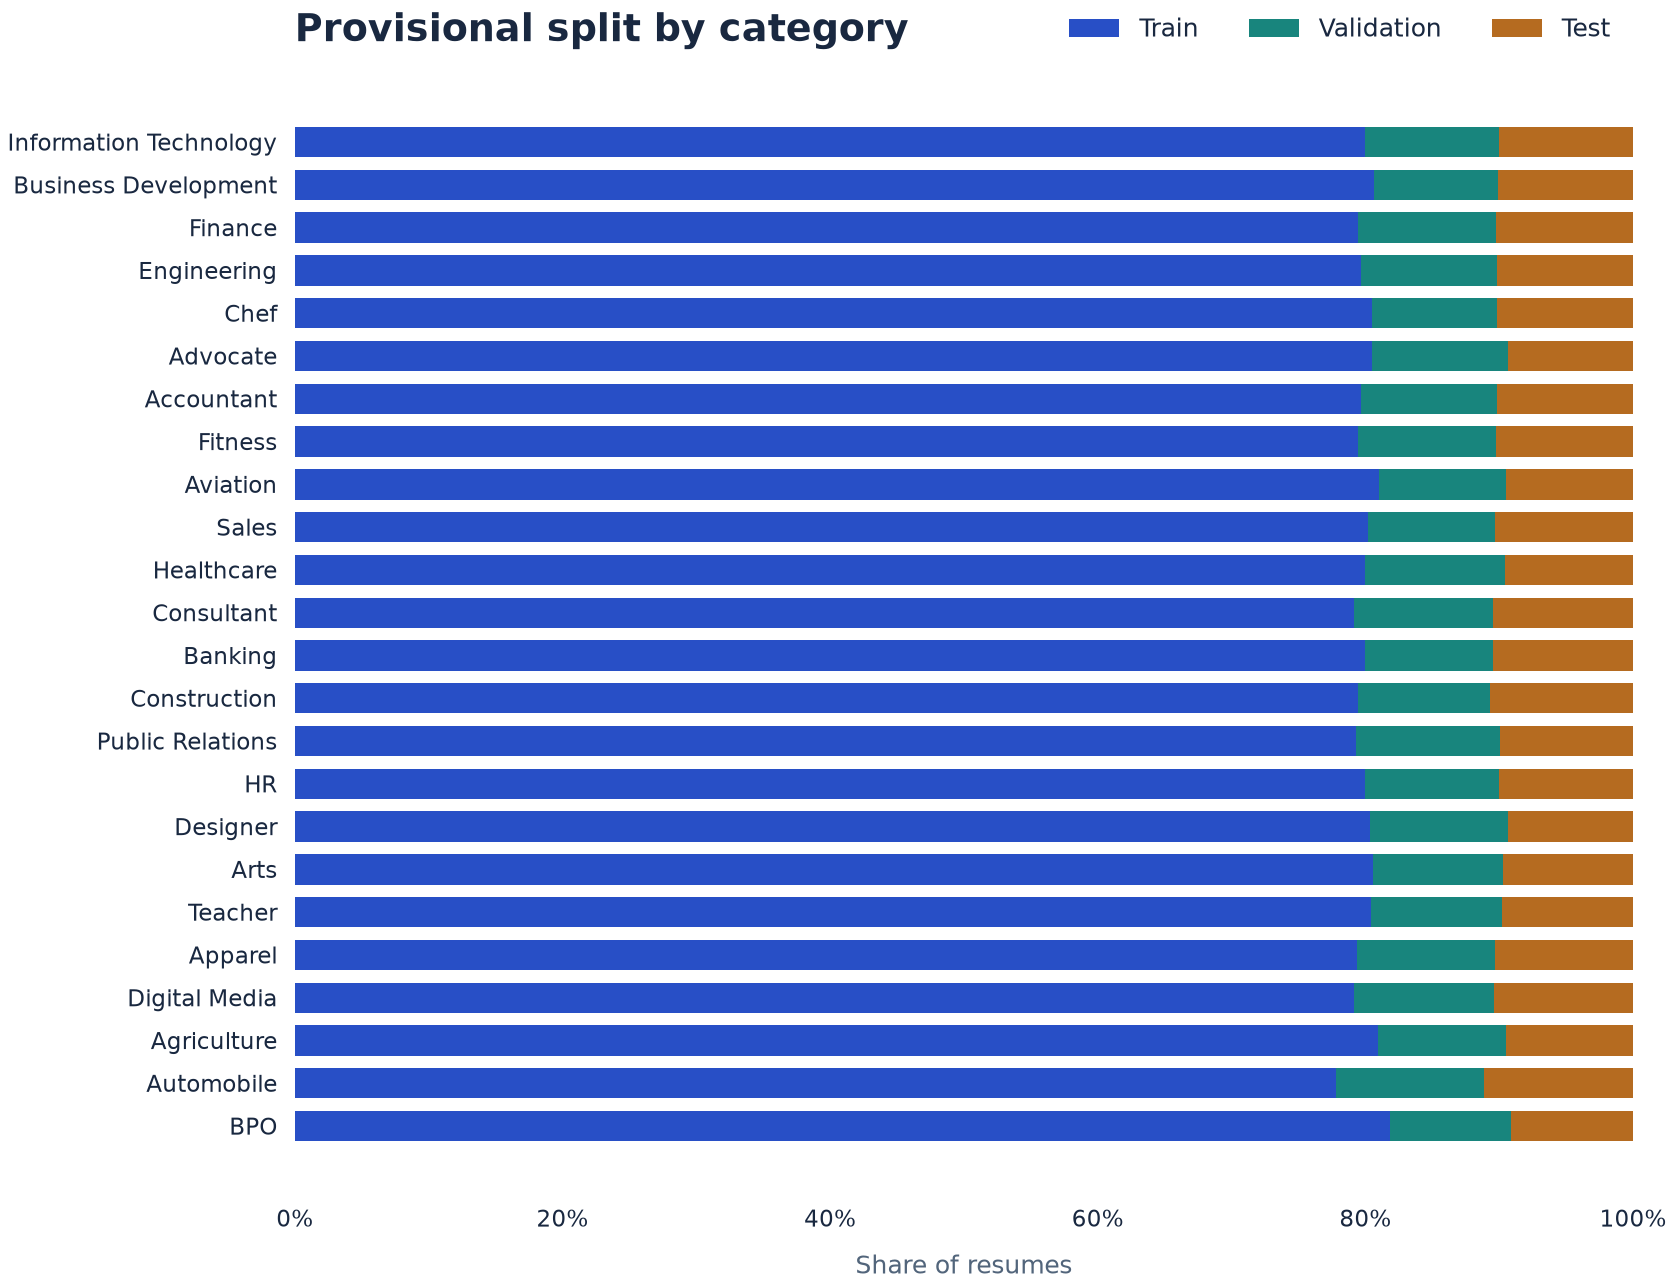
\includegraphics[width=0.92\linewidth]{charts/split_by_category.png}
\caption{Train, validation, and test proportions across all 24 categories.}
\label{fig:split_by_cat}
\end{figure}

In terms of document length, Figure~\ref{fig:length_dist} shows the overall distribution of whitespace-delimited word counts per resume: the \textbf{median} length is \textbf{757 words}, and the \textbf{95th percentile} is \textbf{1,399 words}, with a long right tail extending past 2,000 words. Because subword tokenization (WordPiece) splits words into even more tokens, the vast majority of resumes exceed DistilBERT's 512-token input limit (affecting 89.67\% of training CVs) as well as standard 512-token RNN/CNN sequence budgets—directly motivating the \textbf{Head+Tail truncation} strategy used in downstream modeling. Figure~\ref{fig:length_by_cat} further breaks down word counts by category using boxplots, showing that median lengths are broadly comparable across domains (roughly 650--900 words), with \code{BPO} and \code{INFORMATION-TECHNOLOGY} tending toward slightly longer CVs and \code{SALES} and \code{TEACHER} slightly shorter ones.

\begin{figure}[H]
\centering
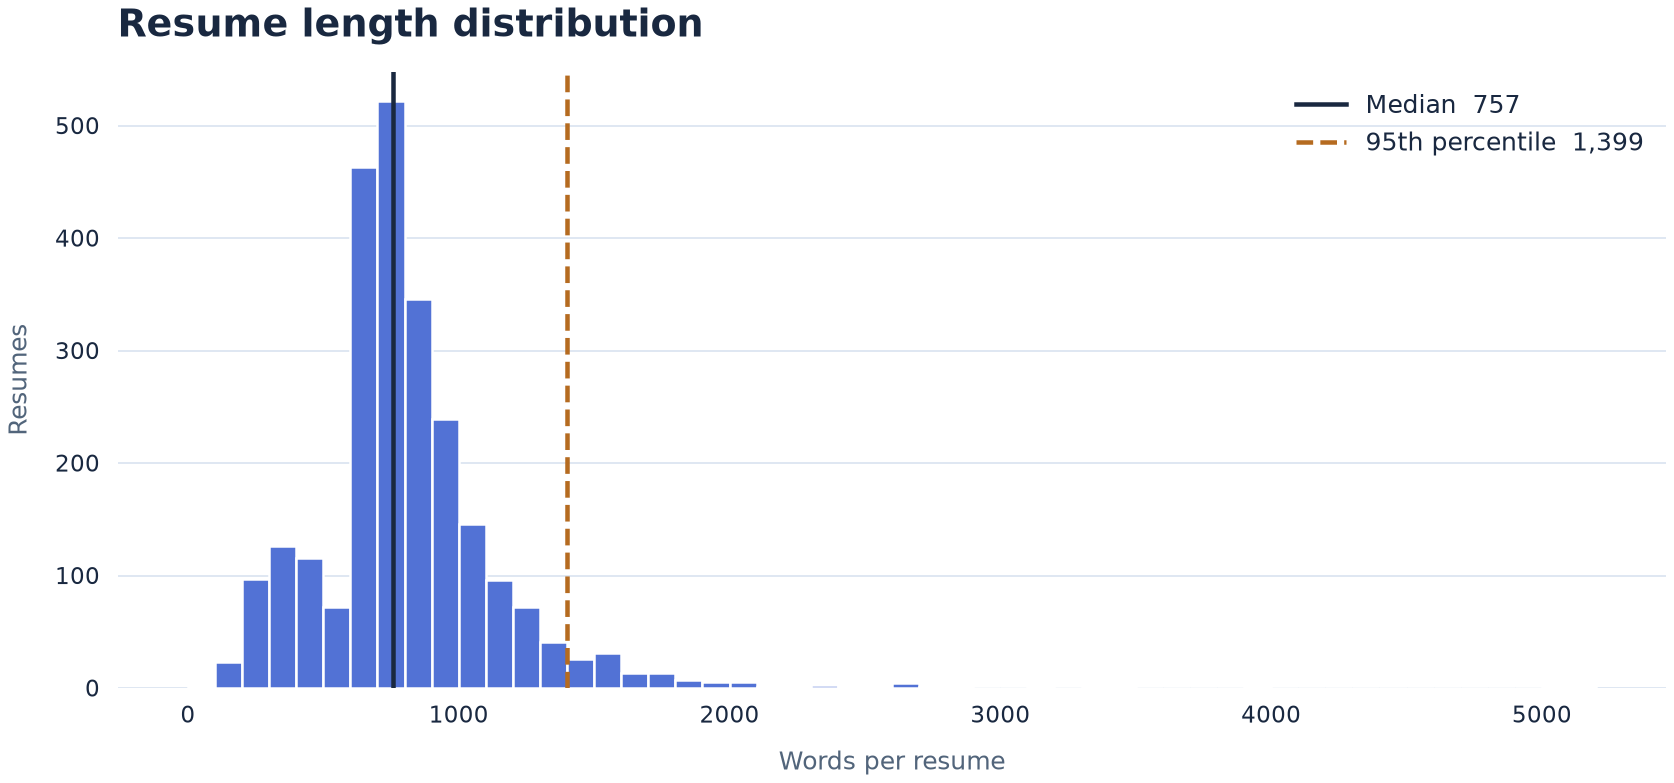
\includegraphics[width=0.88\linewidth]{charts/resume_length_distribution.png}
\caption{Overall resume word-count distribution (median = 757 words, 95th percentile = 1,399 words).}
\label{fig:length_dist}
\end{figure}

\begin{figure}[H]
\centering
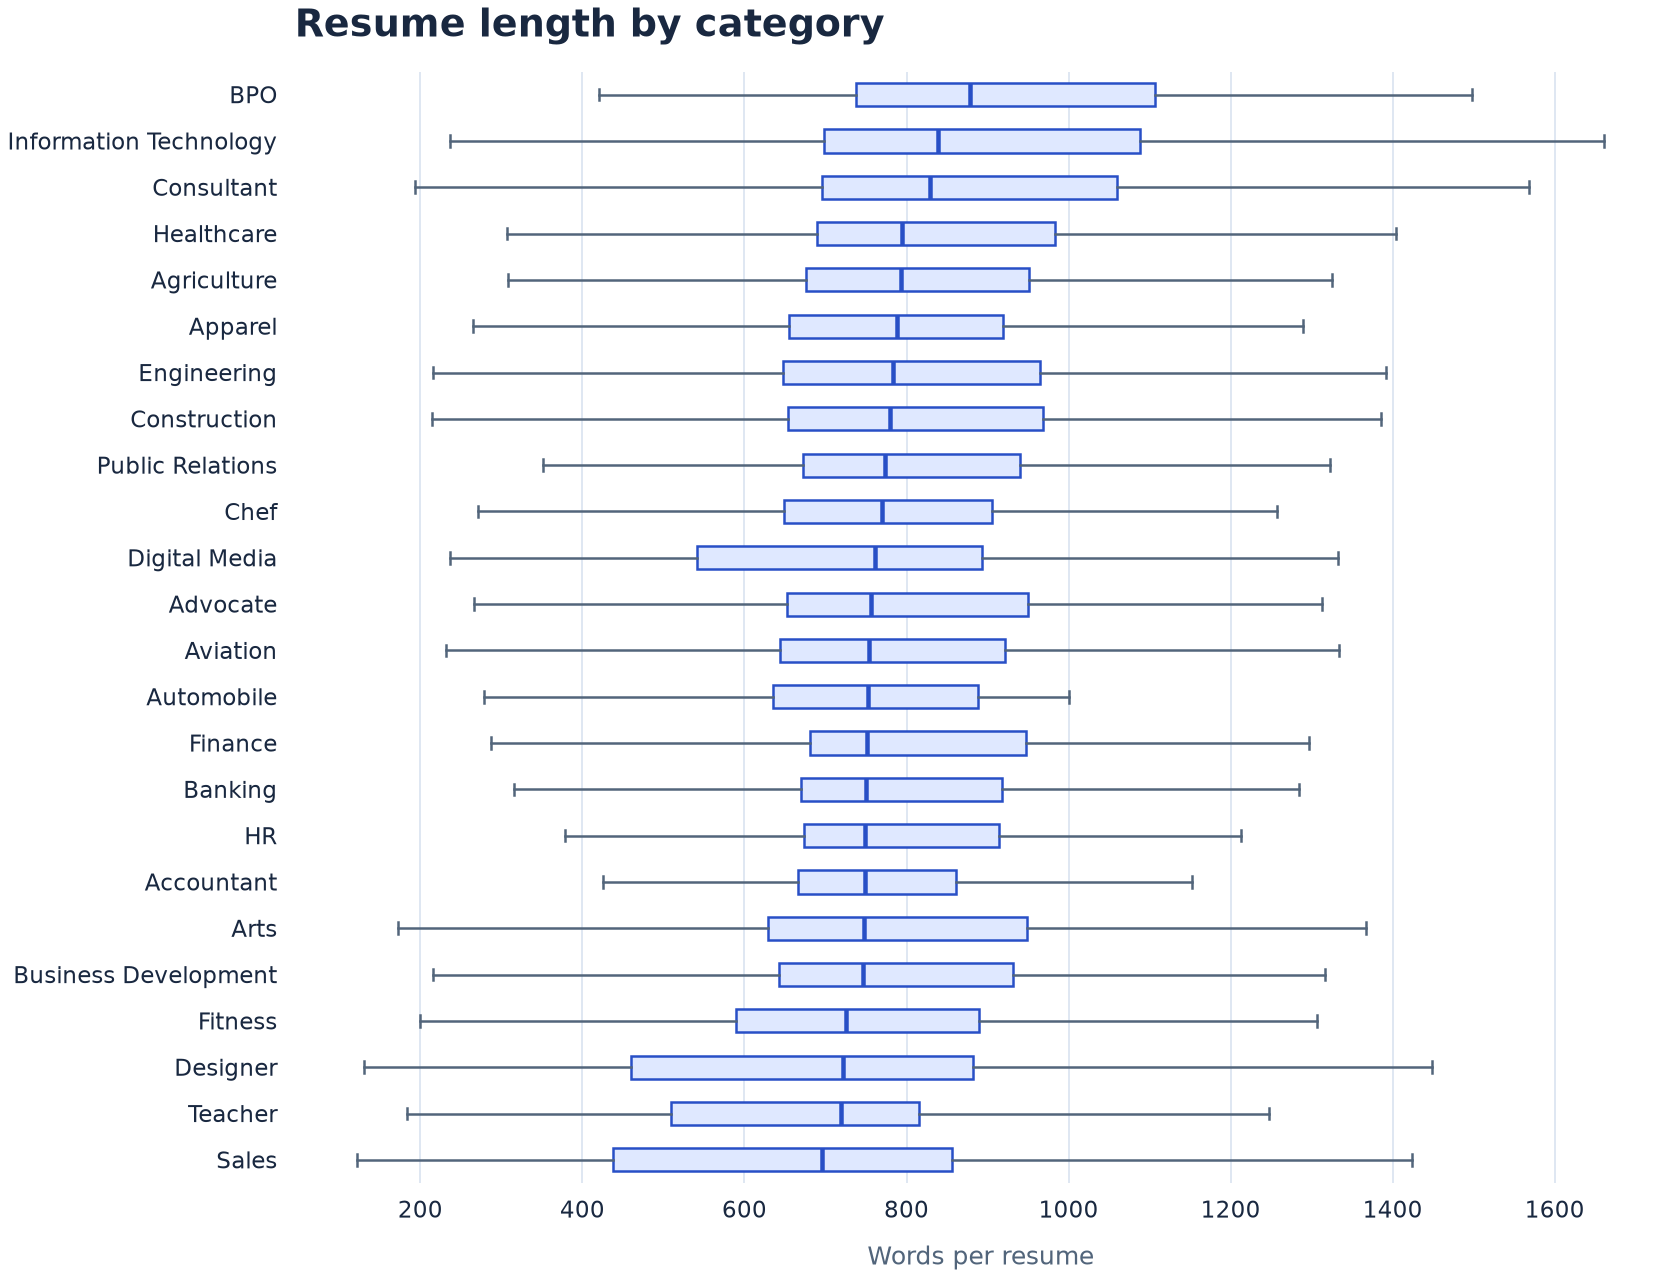
\includegraphics[width=0.92\linewidth]{charts/resume_length_by_category.png}
\caption{Resume word-count distribution by category (boxes span the interquartile range; vertical line marks the median).}
\label{fig:length_by_cat}
\end{figure}

\subsection{Example Samples}
To illustrate how a raw CV appears in the dataset and how each preprocessing stage transforms it, Table~\ref{tab:sample_cv} presents a representative fictional CV example following the exact pipeline rules. Notice how the raw text begins with an explicit uppercase job title (\code{ACCOUNTANT}), includes mixed-case prose with technical skill phrases (\code{Power BI}), and contains personally identifiable contact details (\code{demo@example.com}).

\begin{table}[H]
\centering
\small
\renewcommand{\arraystretch}{1.25}
\begin{tabularx}{\linewidth}{@{}l X@{}}
\toprule
\textbf{Version} & \textbf{CV Text}\\
\midrule
\code{Resume.csv} (raw) & \code{ACCOUNTANT We built Power BI dashboards and managed monthly reports. Email: demo@example.com}\\
\code{raw_no_header.csv} & \code{We built Power BI dashboards and managed monthly reports. Email: demo@example.com}\\
\code{light.csv} & \code{We built Power BI dashboards and managed monthly reports. Email: CONTACT_EMAIL}\\
\code{classical.csv} & \code{built power_bi dashboards managed monthly reports email contact_email}\\
\code{stemmed.csv} & \code{built power_bi dashboard manag month report email contact_email}\\
\code{lemmatized.csv} & \code{build power_bi dashboard manage monthly report email contact_email}\\
\bottomrule
\end{tabularx}
\caption{Illustration of a CV across the raw and five preprocessed text representations.}
\label{tab:sample_cv}
\end{table}

\section{Methodology}
\subsection{Text Preprocessing \& Header Removal}
The preprocessing pipeline (\texttt{src/long\_\-preprocessing/preprocess.py} and \code{run_pipeline.py}) produces five distinct text representations from the raw data so that downstream models—ranging from sparse linear classifiers to RNN/CNN and Transformer architectures—can be evaluated under consistent, leak-free conditions:

\begin{enumerate}
    \item \textbf{HTML-Based Header Removal (\code{raw_no_header.csv}):} Many resumes in the Kaggle dataset open with an explicit job-title header matching or closely resembling the ground-truth \code{Category} label. Rather than blindly stripping the first line of plain text (which risks deleting genuine experience or summary lines when a CV lacks a title), our parser inspects \code{Resume_html} for header CSS classes (\code{name}, \code{resumetitle}, \code{exampletitle}, \code{name-sec}, \code{namesec}, \code{inheader}, \code{name-line}) and aligns the extracted header prefix against the beginning of \code{Resume_str}. The matched prefix is stripped only when sufficient body text remains. As shown in Figure~\ref{fig:header_removal}, out of 2,484 resumes, \textbf{2,444} (98.4\%) had an aligned opening header removed; in \textbf{1,549} cases (62.4\% of all resumes), the removed header contained the literal category phrase, while only \textbf{40} resumes (1.6\%) retained the original text. This \code{text_no_header} output powers the controlled job-title leakage experiment across all model families.

    \item \textbf{Light Cleaning (\code{light.csv}):} Built directly from \code{raw_no_header}, this representation applies NFKC Unicode normalization, standardizes line breaks, bullet symbols, and whitespace, repairs known encoding artifacts (mojibake punctuation) and PDF layout word-splits (e.g., \code{M onitored} $\rightarrow$ \code{Monitored}, \code{d evelop} $\rightarrow$ \code{develop}, \code{con tracts} $\rightarrow$ \code{contracts}), and masks personally identifiable information (PII) into standardized tokens: \code{CONTACT_EMAIL}, \code{CONTACT_URL}, and \code{CONTACT_PHONE} (covering NANP, labeled, and international phone formats). Stop-word removal and stemming are deliberately omitted here: neural architectures (BiLSTM/BiGRU, TextCNN) and pretrained Transformers (DistilBERT) rely on natural word order, prepositions, and casing to preserve contextual semantics consistent with pretraining.

    \item \textbf{Classical Normalization (\code{classical.csv}):} Built from \code{light}, this branch prepares clean tokens for sparse bag-of-words and TF-IDF models. Standard regex tokenizers strip punctuation and split multi-word phrases, which would corrupt technical terms (\code{C++} and \code{C#} collapsing to \code{c}, or \code{Power BI} splitting into generic tokens). Therefore, skill aliases are standardized into single tokens (e.g., \code{C++} $\rightarrow$ \code{cplusplus}, \code{C#} $\rightarrow$ \code{csharp}, \code{ASP.NET} $\rightarrow$ \code{asp_dotnet}, \code{.NET} $\rightarrow$ \code{dotnet}, \code{Node.js} $\rightarrow$ \code{nodejs}, \code{Power BI} $\rightarrow$ \code{power_bi}, \code{Machine Learning}/\code{ML} $\rightarrow$ \code{machine_learning}), text is lowercased and tokenized, and English stop words are removed while explicitly retaining negations (\code{no}, \code{nor}, \code{not}, \code{cannot}) and single-letter programming languages (\code{c}, \code{r}, \code{go}) that default stop-word lists would otherwise discard.

    \item \textbf{Stemming (\code{stemmed.csv}):} Built from \code{classical} by applying NLTK's Snowball \texttt{EnglishStemmer} to reduce vocabulary sparsity by grouping morphological variants (e.g., \code{managed} $\rightarrow$ \code{manag}) while keeping standardized skill and contact tokens intact.

    \item \textbf{Lemmatization (\code{lemmatized.csv}):} Built as a separate branch from \code{light} using spaCy's \code{en_core_web_sm} pipeline for POS-aware lemmatization (e.g., \code{built} $\rightarrow$ \code{build}), followed by skill standardization and stop-word filtering. Unlike rule-based stemming, lemmatization preserves valid dictionary forms at higher computational cost, enabling direct comparison between normalization strategies.
\end{enumerate}

Figure~\ref{fig:header_removal} and Figure~\ref{fig:preproc_lengths} summarize the header-removal coverage and the resulting median and 95th-percentile word counts across all six text versions. Removing stop words in the classical, stemmed, and lemmatized branches reduces median CV length from $\sim$757 words down to $\sim$550--570 words while retaining domain-specific skill and action terms.

\begin{figure}[H]
\centering
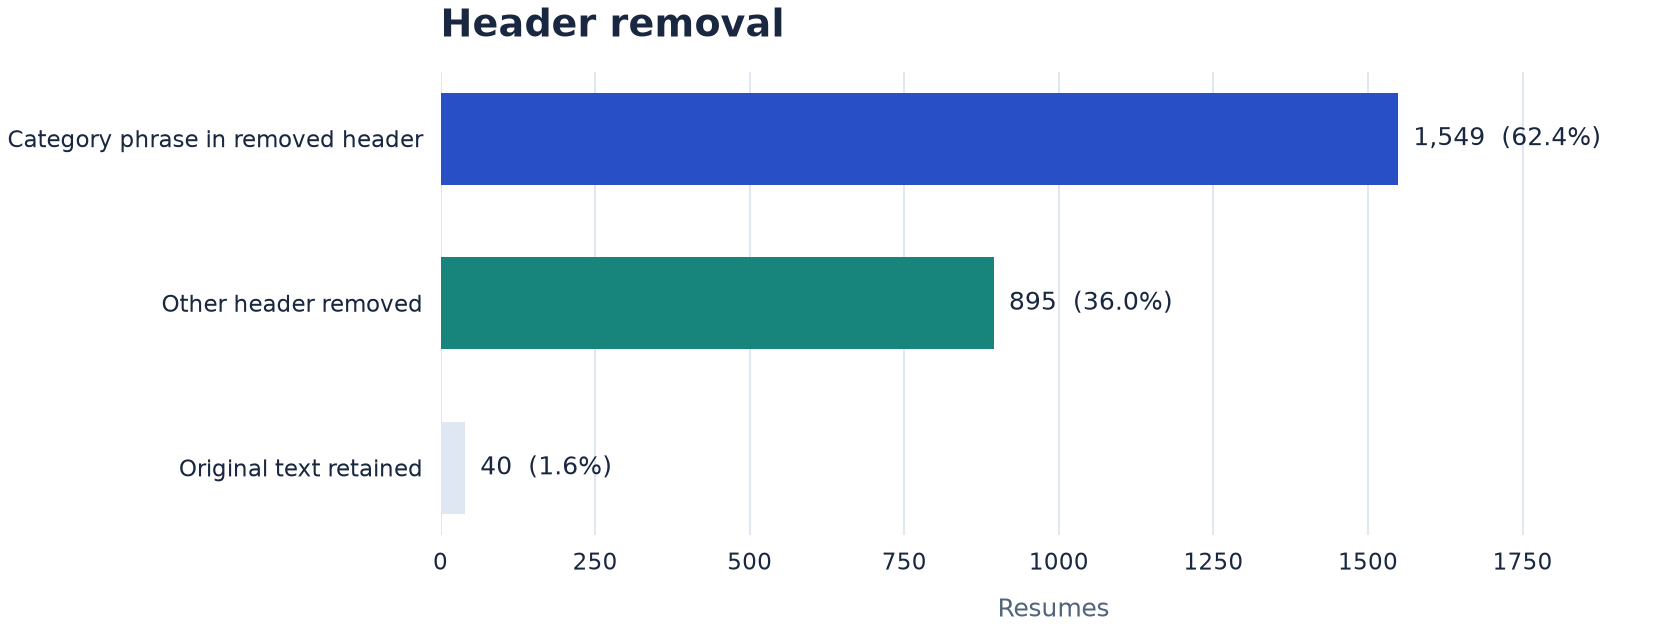
\includegraphics[width=0.88\linewidth]{charts/header_removal.png}
\caption{Summary of HTML-aligned opening header removal across all 2,484 resumes.}
\label{fig:header_removal}
\end{figure}

\begin{figure}[H]
\centering
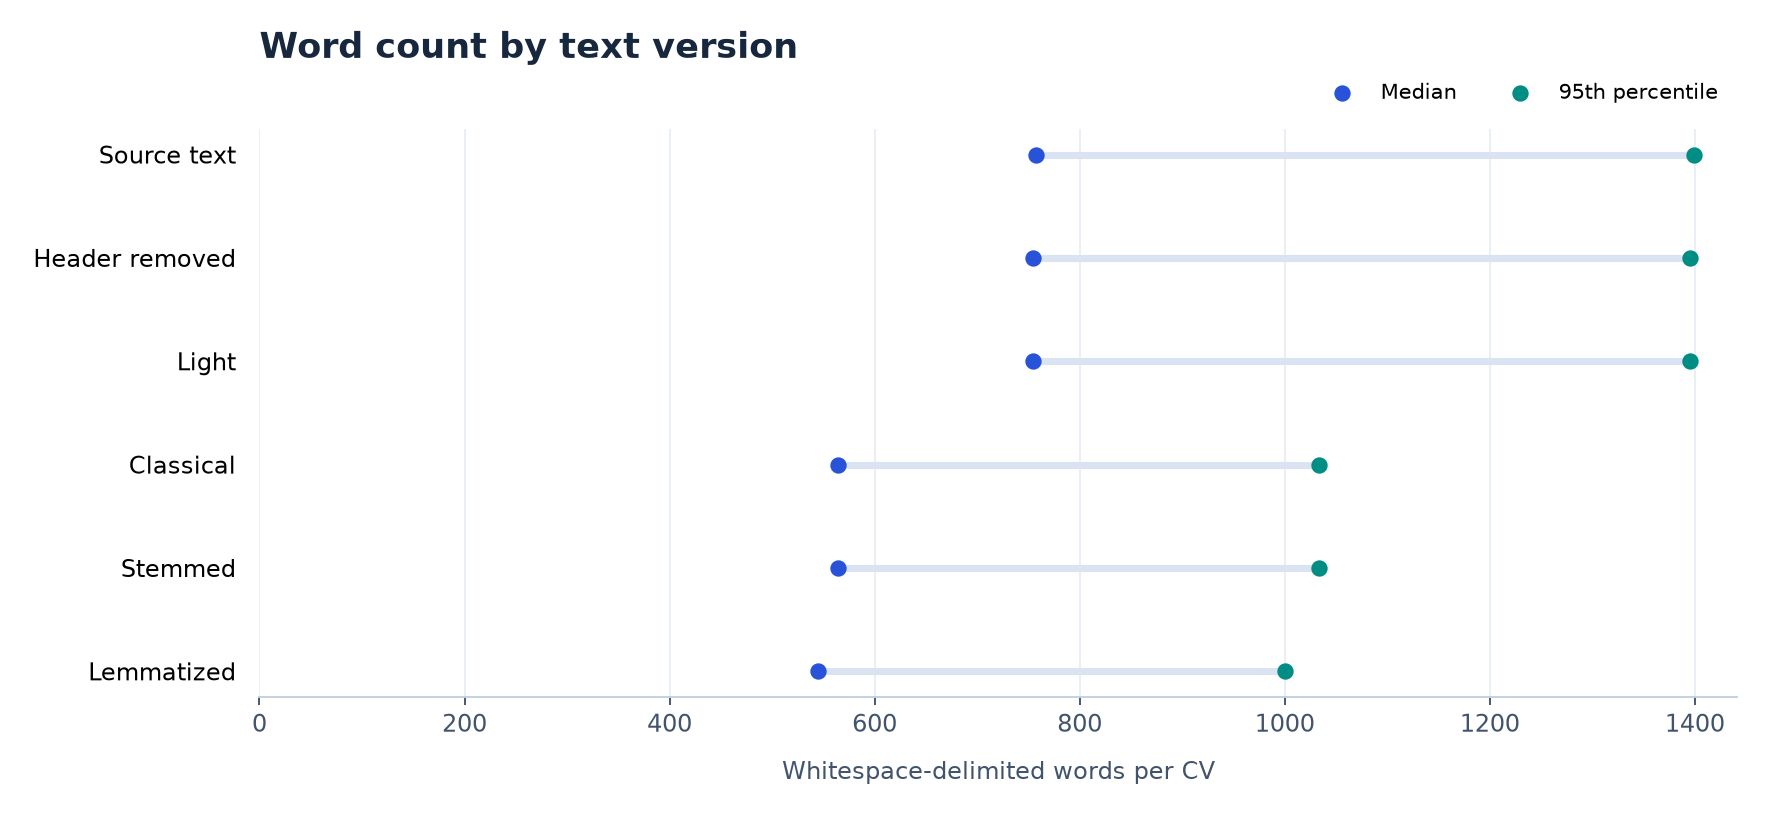
\includegraphics[width=0.88\linewidth]{charts/preprocessing_lengths.png}
\caption{Median and 95th-percentile whitespace-delimited word counts across text preprocessing versions.}
\label{fig:preproc_lengths}
\end{figure}

\subsection{Text Representation Methods}
\par\noindent\textit{[TODO: Describe BoW, TF-IDF, GloVe 300d embeddings, and WordPiece tokenization with Head+Tail truncation.]}

\subsection{Classification Models}
\par\noindent\textit{[TODO: Describe the classical ML baselines (Dummy, Multinomial NB, Logistic Regression, LinearSVC), deep learning models (TextCNN, BiLSTM/BiGRU with attention, CNN+BiLSTM), and fine-tuned DistilBERT.]}

\subsection{Evaluation Metrics \& Protocol}
\par\noindent\textit{[TODO: Describe Accuracy, Macro-Precision, Macro-Recall, Macro-F1, Weighted-F1, Top-3 Accuracy, and why Macro-F1 is the primary metric.]}

\section{Experiments}
\subsection{Experimental Setup \& Data Splitting}
\par\noindent\textit{[TODO: Describe the stratified 80/10/10 train/validation/test split (seed 42) and shared evaluation protocol.]}

\subsection{Hyperparameter Configurations \& Training Details}
\par\noindent\textit{[TODO: Summarize hyperparameter search spaces, training schedules, hardware/runtime environment, and early stopping criteria.]}

\subsection{Controlled Ablations \& Leakage Study}
\par\noindent\textit{[TODO: Describe the job-title removal experiment, representation/architecture ablations, and multi-seed stability runs.]}

\section{Results}
\subsection{Overall Model Comparison}
\par\noindent\textit{[TODO: Present main comparison tables and charts across all classical, deep learning, and Transformer models.]}

\subsection{Job-Title Leakage Analysis}
\par\noindent\textit{[TODO: Present with-title vs. no-title results and analyze the performance drop across model families.]}

\subsection{Seed Stability \& Ablation Results}
\par\noindent\textit{[TODO: Present multi-seed mean $\pm$ std results and key ablation findings.]}

\section{Error Analysis}
\subsection{Per-Class Performance \& Confused Pairs}
\par\noindent\textit{[TODO: Present per-class F1 scores, confusion matrix insights, and most frequently confused category pairs.]}

\subsection{Qualitative Error Breakdown}
\par\noindent\textit{[TODO: Categorize test errors (e.g., dataset label noise vs. genuine model confusion) with concrete examples.]}

\section{Conclusion}
\subsection{Summary of Findings}
\par\noindent\textit{[TODO: Summarize the main takeaways and best-performing pipeline.]}

\subsection{Limitations \& Future Work}
\par\noindent\textit{[TODO: Discuss current limitations and potential future improvements.]}

\section{Task Allocation \& Contribution}
\par\noindent\textit{[TODO: Fill in each member's student ID, assigned tasks, and contribution percentage (summing to 100\%).]}

\begin{table}[H]
\centering
\small
\renewcommand{\arraystretch}{1.35}
\begin{tabularx}{\linewidth}{@{}c p{3.8cm} c X c@{}}
\toprule
\textbf{No.} & \textbf{Full Name} & \textbf{Student ID} & \textbf{Assigned Tasks} & \textbf{Contribution (\%)}\\
\midrule
1 & Kriti Sharma & {[Student ID]} & {[TODO]} & {[\%]} \\
2 & Nguyễn Hà Bảo Phúc & {[Student ID]} & {[TODO]} & {[\%]} \\
3 & Phạm Trương Hoàng Long & 2452700 & {[TODO]} & {[\%]} \\
4 & Yuvaan Chottani & {[Student ID]} & {[TODO]} & {[\%]} \\
\bottomrule
\end{tabularx}
\caption{Team task allocation and contribution breakdown.}
\end{table}

\end{document}
